%% ===================================================================
\section{Real Hospital Networks}\label{sec:real}

The simulations control everything; real data control nothing. This section asks whether GHB's advantages survive real hospitals, real heterogeneity and real sample sizes, against the federated and personalized methods that apply, at the same privacy budget. It reports two studies. The first is a confirmation on networks that no part of GHB's development had seen. Its rule, its predictions and the frozen configuration of every method were committed to the repository before it ran (Section~\ref{sec:real-tcga}). The second is the earlier benchmark of eight smaller networks, on which GHB-lite was developed and its limits were found (Section~\ref{sec:real-eight}). The design of GHB in Section~\ref{sec:logit} came out of those limits, and every step of that development is reported, including the two pre-registered attempts that failed.

\subsection{A pre-registered test on unseen networks}\label{sec:real-tcga}

\paragraph{Networks and model} The Cancer Genome Atlas \cite{weinstein2013cancer,grossman2016toward} records, for every patient, the institution that contributed the tissue. Each cancer type is a network, and each institution with at least five eligible patients is a hospital. The outcome is death within two years of diagnosis; patients alive with less than two years of follow-up are excluded. Every hospital fits a logistic regression with eight coefficients: intercept, age, sex, pathologic stage III, stage IV, tumour stage T3 or T4, nodal involvement and a prior malignancy, with $\|x\|\le\sqrt{8}$ by construction (FIGO stage replaces the AJCC stage for the gynecologic cancers). Twelve networks served for development: lung squamous and adenocarcinoma, head and neck, bladder, stomach, liver, clear-cell and papillary kidney, colon, rectum, pancreas and oesophagus (5 to 17 hospitals each). The confirmation set was then fixed by a rule on counts alone, before any model was fitted to it. It contains every further TCGA project with at least four such hospitals and at least fifteen deaths: breast (8 hospitals), mesothelioma (9), ovarian (15), endometrial (15) and uterine carcinosarcoma (5). Hospitals hold 5 to 109 eligible patients.

\paragraph{Protocol} Every hospital is evaluated on its own held-out patients by ten repetitions of stratified five-fold cross-validation, and errors are held-out log-loss relative to local estimation under the default prior $\mathcal{N}(0,2.5^2)$. Every private method spends the same budget, $\epsilon\in\{1,10\}$ with $\delta=10^{-5}$ under zero-concentrated accounting. The literature methods are DP-FedAvg with local fine-tuning, with and without secure aggregation; clustered DP-FedAvg; APFL; Ditto \cite{li2021ditto}; and pFedMe \cite{tdinh2020personalized}. Each has a grid of 18 to 54 configurations, and how it is tuned decides how it compares. In the \emph{realistic} arm, each method uses the configuration with the lowest mean error over the twelve development networks, frozen before the confirmation. This is what a consortium could do with networks it already has. In the \emph{oracle} arm, each method uses the configuration that is best on the confirmation network's own held-out folds, which no hospital can do. GHB is not tuned: its configuration (Section~\ref{sec:logit}) was chosen among about fifteen variants on the development networks and frozen together with the baselines'. The two privacy budgets bracket the regime of interest. At $\epsilon=1$ the joint releases of a network of a few hundred patients are noisy. At $\epsilon=10$ they are accurate, and borrowing can pay.

\paragraph{How GHB was developed} GHB-lite, with an evidence-weighted default prior, was the starting point. On the twelve development networks it is no better than a local model with the same prior at $\epsilon=1$ (\SimTDOneLite{} against \SimTDOneLoc), and worse at $\epsilon=10$ (\SimTDTenLite{}). A pre-registered extension of GHB-lite added four components: a no-borrowing option, a network-learned prior scale, correlated heterogeneity and borrowing across cancer types. It was confirmed on six networks that were then unseen. Its predictions held, but at $\epsilon=10$ every variant was worse than local estimation, which the extension was meant to prevent; that confirmation made those six networks part of the development set. The diagnosis was the bias and the noise of GHB-lite's per-hospital releases (Section~\ref{sec:logit}), and GHB replaces them by the two joint releases. On the development networks GHB reaches \SimTDOneGHB{} at $\epsilon=1$ and \SimTDTenGHB{} at $\epsilon=10$, against \SimTDOneBestLit{} and \SimTDTenBestLit{} for the best literature method tuned on the same networks. The ablation in the supplement removes one component at a time. Borrowing across cancer types and propagating the privacy covariance matter most, at both budgets (without them the mean error rises by 0.007 to 0.035). Each of the other components changes it by less than 0.007.

\begin{table}[t]
\caption{Pre-registered confirmation on five TCGA networks that no part of the development had seen (hospitals: BRCA 8, MESO 9, OV 15, UCEC 15, UCS 5): held-out log-loss relative to local estimation under the default prior (ten repetitions of five-fold cross-validation). GHB and GHB-lite have nothing to tune. Every literature method uses the configuration that is best on the twelve development networks, frozen before this run. Bold: the lowest per network among methods that use other hospitals, oracle excluded. Wins: networks in which GHB is more accurate. $\ddagger$: no other hospital. $\star$: for each network, the best configuration of the best of the six methods on that network's own held-out folds, which no hospital can do.}
\label{tab:tcga-confirm}
\scriptsize
\setlength{\tabcolsep}{4pt}
\begin{tabular}{@{}lrrrrrrr@{}}
\toprule
Method & BRCA & MESO & OV & UCEC & UCS & Mean & Wins\\
\midrule
\csname @@input\endcsname ../Collectively_Big_Locally_Small/supplement/results/tables/t_tcga_confirm.tex 
\bottomrule
\end{tabular}
\end{table}

\paragraph{Predictions and outcome} The pre-registration made three predictions, and all three held (Table~\ref{tab:tcga-confirm}).
\begin{itemize}[leftmargin=*]
\item \emph{GHB has a lower mean error than every literature method in the realistic arm, at both budgets.} At $\epsilon=1$, GHB reaches \SimTCOneGHB{}, against \SimTCOneFT{} for the best of them, DP-FedAvg with fine-tuning, and between \SimTCOneClu{} and \SimTCOnePFedMe{} for the others. At $\epsilon=10$, GHB reaches \SimTCTenGHB{}, against \SimTCTenDitto{} for Ditto and \SimTCTenPFedMe{} for pFedMe; the other four reach between \SimTCTenFT{} and \SimTCTenFTSA.
\item \emph{At $\epsilon=10$ GHB improves on GHB-lite.} It does, from \SimTCTenLite{} to \SimTCTenGHB.
\item \emph{At $\epsilon=10$ GHB beats the best realistic method in at least three of the five networks.} It beats Ditto in exactly \SimTCTenDittoWins, and every other method in at least four.
\end{itemize}

\paragraph{Against the oracle} GHB was also more accurate than local estimation at both budgets, which GHB-lite was not. Against the oracle arm, which the pre-registration made no prediction about, the picture depends on the budget. At $\epsilon=1$, GHB has a lower mean error than every one of the six methods even when each is tuned on the test folds (\SimTCOneFTOrc{} for the best of them). Only the best method chosen afresh for each network comes close (\SimTCOneBestOrc). At $\epsilon=10$, GHB ties DP-FedAvg with fine-tuning tuned on the test folds (\SimTCTenFTOrc), and is slightly behind Ditto (\SimTCTenDittoOrc) and DP-FedAvg with secure aggregation (\SimTCTenFTSAOrc). It is clearly behind pFedMe (\SimTCTenPFedMeOrc), and behind the best method chosen afresh for every network (\SimTCTenBestOrc). These are the margins that tuning on a hospital's own test patients buys. A deployment cannot buy them.

\paragraph{What the confirmation supports} Five networks are a small sample. At $\epsilon=10$ the margin over Ditto is small enough, \SimTCTenDitto{} against \SimTCTenGHB{} with three wins in five, that a different set of networks could reverse it. The claim the confirmation supports is therefore specific. Without any tuning, on networks it had not seen, GHB was more accurate than every federated and personalized method tuned in the way a consortium could tune it, at both budgets. Under strong privacy, it was more accurate than every one of them even with tuning that no consortium has. It does not support the claim that GHB dominates the literature in every network or under every way of tuning.

\subsection{Eight smaller networks}\label{sec:real-eight}


\paragraph{Eight real networks} All data are public and need no credentials. \emph{Arizona Medicare} \cite{hilbe2011negative}: 1,466 admissions for percutaneous cardiovascular procedures at 43 hospitals with at least five patients (median 29), in-hospital death (34\%), predictors age 80 or over, HMO membership, urgent and emergency admission. \emph{The Cancer Genome Atlas} \cite{weinstein2013cancer,grossman2016toward}: six networks, one per cancer type (lung squamous, head and neck, bladder, stomach, liver and clear-cell kidney carcinoma), each hospital the tissue source site that contributed its patients (7 to 17 hospitals, median 11 to 29 patients), death within two years of diagnosis, predictors age, sex, and pathologic stage III and IV. \emph{UCI Heart Disease} \cite{detrano1989international}: the four hospitals described below, used as the development network. With four or five coefficients and a few dozen patients per hospital these networks hold little to share, which is the setting of siloed smallness and also the hardest one for any collaborative method.

\paragraph{Protocol} Every hospital is evaluated on its own held-out patients by repeated stratified five-fold cross-validation (100 splits per network), and errors are reported as held-out log-loss relative to local estimation with the default prior. Every private method spends the same budget per hospital, $\epsilon\in\{1,10\}$ and $\delta=10^{-5}$, with zero-concentrated accounting. GHB runs without an anchor, because no published model is assumed, and inverts its releases with a nominal public feature distribution fixed before the data were seen. Twelve literature methods are compared: DP-FedAvg alone and with local fine-tuning, with and without secure aggregation; decentralized DP-SGD; clustered DP-FedAvg; a one-shot Ditto-style model; and the personalized methods Ditto \cite{li2021ditto}, pFedMe \cite{tdinh2020personalized}, APFL, Per-FedAvg \cite{fallah2020personalized}, FedRep \cite{collins2021exploiting} and FedProx \cite{li2020federated}, each with private gradients under the same accounting (SCAFFOLD and FedProx with one full-batch local step coincide with DP-FedAvg). Each has a grid of hyperparameters, and how it is tuned decides how it compares. Three tuning arms are reported. \emph{Oracle}: tuned on each network's own held-out folds, an upper bound no hospital can reach. \emph{Leave-one-network-out}: the configuration with the lowest mean error on the other seven networks, the most generous tuning a hospital could actually do. \emph{Development}: tuned on UCI Heart Disease alone and frozen. GHB-EB has nothing to tune. Two local-only references separate what collaboration contributes from what regularization does: local estimation with a tuned prior scale, and local gradient descent with a tuned number of steps.

\begin{figure}[t]
\centering
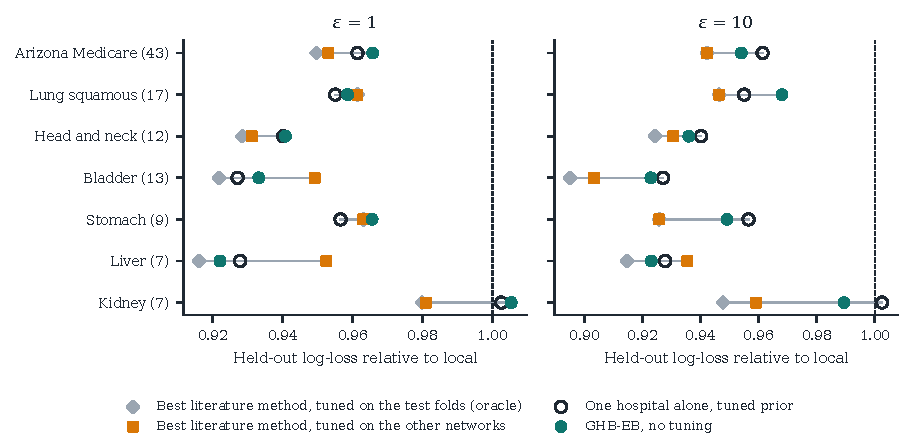
\includegraphics[width=\linewidth]{supplement/figures/real_final}
\caption{Seven real networks (hospitals in parentheses): held-out log-loss relative to local estimation, at $\epsilon=1$ and $\epsilon=10$. Teal: GHB-EB, which has nothing to tune. Orange: the best of twelve federated and personalized methods for that network, each tuned on the other seven networks. Grey: the same, tuned on the network's own held-out folds (oracle). Open circle: one hospital alone with a tuned prior. Choosing the best of twelve methods separately for every network is itself an advantage no hospital has.}
\label{fig:real-final}
\end{figure}

\begin{table}[t]
\caption{Seven real networks: held-out log-loss relative to local estimation, mean over the networks, for every method in the oracle arm (tuned on the network's own held-out folds) and the leave-one-network-out arm (tuned on the other networks); Wins: in how many of the seven networks GHB-EB, untuned, has a lower error than that method in the leave-one-network-out arm. $\ddagger$: no other hospital. Every method spends the same budget. Per-network values are in the supplement.}
\label{tab:real-final}
\scriptsize
\setlength{\tabcolsep}{4pt}
\begin{tabular}{@{}lrrrrrr@{}}
\toprule
 & \multicolumn{3}{c}{$\epsilon=1$} & \multicolumn{3}{c}{$\epsilon=10$}\\
\cmidrule(lr){2-4}\cmidrule(l){5-7}
Method & Oracle & Other networks & Wins & Oracle & Other networks & Wins\\
\midrule
\csname @@input\endcsname ../Collectively_Big_Locally_Small/supplement/results/tables/t_real_final.tex 
\bottomrule
\end{tabular}
\end{table}

\paragraph{With strong privacy, collaboration adds little for anyone} At $\epsilon=1$ (Figure~\ref{fig:real-final}, Table~\ref{tab:real-final}) GHB-EB, untuned, reduces the error of local estimation to \SimRFOneEB{} on average (\SimRFOneEBMin{} to \SimRFOneEBMax{} across networks). Tuned on the other networks, no literature method does better on average: the closest are Ditto (\SimRFOneDittoLono) and pFedMe (\SimRFOnePFedMeLono), and GHB-EB has a lower error than each of the twelve methods in at least four of the seven networks. Tuned on each network's own test folds, DP-FedAvg with fine-tuning and secure aggregation reaches \SimRFOneFTSAOrc, and the best of the twelve methods chosen afresh for every network beats GHB-EB in all but \SimRFOneBestOrcWins. But a single hospital that simply regularizes well does as well as any collaborative method: local estimation with a tuned prior reaches \SimRFOneLocLono, and GHB-EB is better than it in only \SimRFOneEBvsLocWins{} network. At this budget the privacy noise of each release is many times a hospital's own sampling error (Section~\ref{sec:heart-size} below), so the information these networks could share is mostly lost, whatever the method; what remains is regularization, which every method obtains in its own way.

\paragraph{With weaker privacy, the best tuned baselines lead by less than one percent} At $\epsilon=10$, collaboration starts to pay: GHB-EB (\SimRFTenEB) is better than local estimation with a tuned prior in \SimRFTenEBvsLocWins{} of the seven networks. Tuned on the other networks, pFedMe (\SimRFTenPFedMeLono) and DP-FedAvg with fine-tuning and secure aggregation (\SimRFTenFTSALono) are slightly more accurate on average than GHB-EB, Ditto ties it (\SimRFTenDittoLono), and the other nine methods are less accurate. Tuned on the test folds, DP-FedAvg with fine-tuning and secure aggregation leads by about two percent (\SimRFTenFTSAOrc).

\paragraph{Tuning is most of the baselines' advantage} The comparison turns on how the literature methods are tuned, and GHB has nothing to tune. Every baseline loses accuracy when its settings must come from other networks, and several become unstable: tuned on UCI Heart Disease alone, the mean error at $\epsilon=1$ becomes \SimRFOneFTSAUci{} for DP-FedAvg with fine-tuning and secure aggregation, \SimRFOneDittoUci{} for Ditto and \SimRFOnePFedMeUci{} for pFedMe, against \SimRFOneEB{} for GHB-EB, and FedRep diverges. A small hospital cannot tune on its own test patients, and has few patients to hold out for validation; the leave-one-network-out arm is the most a consortium could do for it, and there GHB-EB is the most accurate collaborative method at $\epsilon=1$ and within one percent of the best at $\epsilon=10$.

\paragraph{Two improvements, pre-registered} The first real-data run showed GHB, as reported, at the local level (\SimRFOneGHB{} at $\epsilon=1$): its fixed default prior $\mathcal{N}(0,2.5^2)$ is too loose for hospitals of a few dozen patients. \emph{GHB-EB} integrates the scale of the default prior out over $\{0.5,1,2.5\}$, weighting each scale by the hospital's own evidence exactly as $\tau$ is integrated out (Remark~\ref{rem:tau}); it needs no held-out data. It was developed on simulations with separate seeds and on UCI Heart Disease, and pre-registered with two criteria: improve on GHB in at least five of the seven networks, and raise no network's worst-hospital ratio by more than 0.1. It improved on GHB in \SimRFOneEBvsGHBWins{} networks but raised the worst ratio in the liver network from \SimRFOneLiverWorstGHB{} to \SimRFOneLiverWorstEB, through a hospital whose 22 patients all died; by its own rule it is reported as an extension, not as the default. Its gain at $\epsilon=1$ equals that of a local model with the same evidence-weighted prior, so it comes from regularization, not from borrowing. \emph{GHB-SA} replaces the per-hospital releases by two rounds of secure aggregation, so that the noise is added once to network sums whose sensitivity is set by one patient rather than by the smallest hospital. In development it removed about half of the privacy cost (supplement); on the real networks it improved on GHB-EB in only \SimRFOneSAvsEBWins{} of seven at $\epsilon=1$, with a worst ratio of \SimRFOneLiverWorstSA{} in the liver network, and failed its pre-registered criterion. With seven to seventeen hospitals, the heterogeneity statistic that GHB-SA privatizes as a single sum is too noisy, and its nominal public feature distribution biases it; at $\epsilon=10$ it matches GHB-EB (\SimRFTenSA{} against \SimRFTenEB). Both negative outcomes stand in the paper because they bound what GHB can do on networks of this size.

\paragraph{How much the size of a hospital matters}\label{sec:heart-size} The UCI Heart Disease data \cite{detrano1989international} are the classic multi-site benchmark of federated learning in healthcare \cite{ogierduterrail2022flamby}. They hold the records of patients referred for coronary angiography at four hospitals: the Cleveland Clinic (303 patients), the Hungarian Institute of Cardiology in Budapest (294), the University Hospitals of Zurich and Basel (123) and the VA Medical Center in Long Beach (200). The prevalence of angiographic coronary disease ranges from 36\% in Budapest to 93\% in Zurich and Basel, so the heterogeneity is real and large. Each hospital fits the pretest-probability model of coronary disease, a logistic regression on age, sex and chest-pain type (asymptomatic, anginal, or non-anginal as reference), the predictors that every site records completely. Age is scaled by public constants, $(\text{age}-55)/25$ clipped to $[-1,1]$, so that $\|x\|\le\sqrt{5}$ without fitting anything to the data. No published model is assumed, so GHB runs without an anchor: it releases the score at the public point 0, linearizes under the default prior, and gossips on a ring of four hospitals. The public feature distribution needed for the inversion is a nominal chest-pain clinic population (age $\mathcal{N}(55,9^2)$, 75\% men, 50\% asymptomatic, 30\% anginal pain), not the data, so every hospital is under a real case-mix shift. Evaluation is by repeated stratified five-fold cross-validation within each hospital (\SimRealHeartSplits{} splits). Each hospital trains on its training folds, subsampled to at most 20, 40 or 80 patients to emulate siloed smallness, or on all of them, and is scored by log-loss on its own held-out fold. The baselines are the same as in Simulation 15, with their hyperparameters chosen on the held-out folds themselves, which favours them. A local-only control, gradient descent on the hospital's own data with a tuned number of steps, separates what they gain by collaborating from what they gain by regularizing.

The result is mixed, and it is consistent with the theory. At $\epsilon=1$, no private method gains from collaboration in this network. GHB stays within 1\% of local estimation at every training size (\SimRealHeartTwentyGHBRel{} with at most 20 patients, \SimRealHeartAllGHBRel{} with all of them), and its worst hospital stays within a factor \SimRealHeartGHBWorstMax{} of its local error, at $\epsilon=5$ too. The privacy noise explains why. On the parameter scale, a hospital of 40 patients releases noise with a standard deviation about 26 times its own sampling error at $\epsilon=1$, and about 10 times at 300 patients. With only three other hospitals to average over, $M$ in Equation~\eqref{eq:M} dwarfs $\tau^2$ and Equation~\eqref{eq:borrowed} leaves almost nothing to borrow. GHB's posterior over $\tau$ and the hospital's own evidence detect this and fall back to local estimation, without any tuning. The tuned DP-FedAvg with fine-tuning appears to gain (\SimRealHeartTwentyFTRel{} with 20 patients). The local-only control gains exactly as much (\SimRealHeartTwentyLGDRel), because the chosen configuration is a single private round followed by 30 local steps, so its gain is early stopping tuned on the test folds, not borrowing. The Ditto-style model, pulled toward the average of the private releases, fails badly with small hospitals (\SimRealHeartTwentyDittoRel). Without privacy, GHB borrows: \SimRealHeartTwentyGHBNoDPRel{} of the local error with at most 20 training patients, \SimRealHeartFortyGHBNoDPRel{} with 40 and \SimRealHeartEightyGHBNoDPRel{} with 80, fading to \SimRealHeartAllGHBNoDPRel{} with all of them, as Equation~\eqref{eq:borrowed} predicts when $n_k$ grows. The nominal public feature distribution costs nothing: replacing it by the pooled empirical features gives \SimRealHeartTwentyGHBEmpRel{} with 20 patients. A single pooled model, also without privacy, is worse than local estimation on average at every size (\SimRealHeartTwentyGlobalRel{} to \SimRealHeartAllGlobalRel) and makes the Swiss hospital, with its 93\% prevalence, \SimRealHeartGlobalWorstMin{} to \SimRealHeartGlobalWorstMax{} times worse off. GHB without privacy keeps every hospital within 2\% of its local error. The lesson for deployment is the one the theory states. In a network of four hospitals of tens to a few hundred patients, a guarantee of $\epsilon=1$ per release leaves nothing to share, and GHB's value there is that it does no harm. Collaboration under privacy needs more hospitals (Simulation 17), joint release by small hospitals (Section~\ref{sec:privacy}) or a larger budget, and these data, unlike the eICU and similar collections, cannot test the regime of tens of hospitals that the simulations describe.

\begin{figure}[t]
\centering
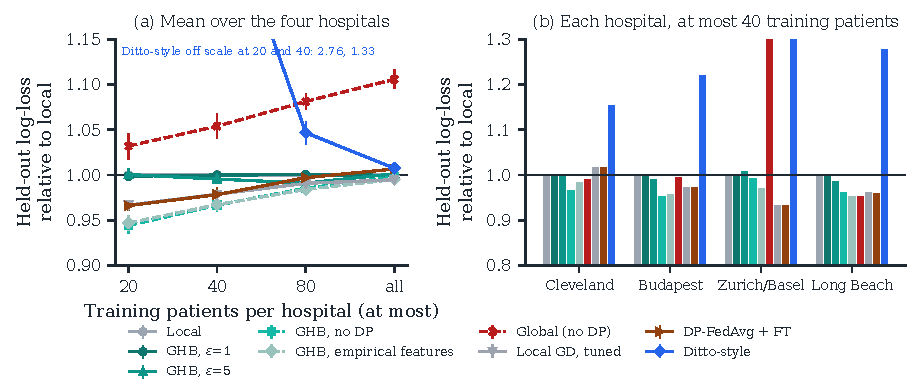
\includegraphics[width=\linewidth]{supplement/figures/real_heart}
\caption{UCI Heart Disease, four hospitals: held-out log-loss relative to local estimation (repeated stratified five-fold cross-validation, \SimRealHeartSplits{} splits; $\pm2$ paired standard errors). (a) Mean over hospitals against the number of training patients per hospital. (b) Each hospital, with at most 40 training patients (bars clipped at 1.3; values in Table~\ref{tab:real-heart} and the supplement). Dashed: without privacy. The baselines' hyperparameters are tuned on the held-out folds.}
\label{fig:real-heart}
\end{figure}

\begin{table}[t]
\caption{UCI Heart Disease: held-out log-loss relative to local estimation (two paired standard errors in grey) and the largest ratio of any hospital's held-out log-loss to its local one (Worst), by the number of training patients per hospital (\SimRealHeartSplits{} splits). First row: local log-loss (nats). DP-FedAvg + FT, Ditto-style and local GD are tuned on the held-out folds. $\dagger$: not private.}
\label{tab:real-heart}
\scriptsize
\setlength{\tabcolsep}{3.5pt}
\begin{tabular}{@{}lrrrrrrrr@{}}
\toprule
 & \multicolumn{2}{c}{$\le 20$ patients} & \multicolumn{2}{c}{$\le 40$} & \multicolumn{2}{c}{$\le 80$} & \multicolumn{2}{c}{All}\\
\cmidrule(lr){2-3}\cmidrule(lr){4-5}\cmidrule(lr){6-7}\cmidrule(l){8-9}
Method & Relative & Worst & Relative & Worst & Relative & Worst & Relative & Worst\\
\midrule
\csname @@input\endcsname ../Collectively_Big_Locally_Small/supplement/results/tables/t_real_heart.tex 
\bottomrule
\end{tabular}
\end{table}

\paragraph{What the real data say} Three findings hold across the eight networks. First, on networks of a few to a few dozen small hospitals with simple models, privacy at $\epsilon=1$ leaves little to share, and a hospital that regularizes well alone is as accurate as any collaborative method; the theory predicts this through Equations~\eqref{eq:M} and~\eqref{eq:borrowed}, and a network can check it from public quantities before it starts. Second, when collaboration does pay, GHB is competitive with the best federated and personalized methods without any tuning, and is the most accurate of them when their tuning must be transferred from other networks; tuned on the test data, which no hospital can do, the best of them lead by one to two percent. Third, the safety property holds where it matters: GHB never makes a hospital much worse off except at a hospital whose data are degenerate, where every method fails, and a single pooled model is the least safe of all methods. The real data do not show GHB dominating the literature, and the paper does not claim it.
